%inspired from: https://tex.stackexchange.com/questions/386345/directed-graph-example-in-tikz
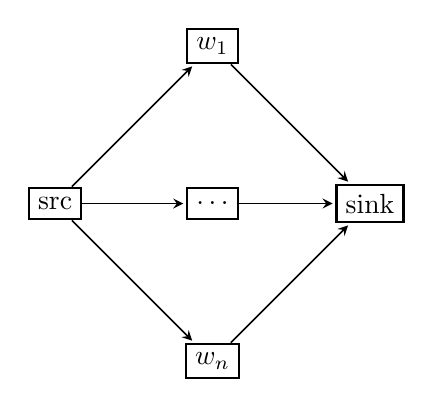
\begin{tikzpicture}[
     > = stealth, % arrow head style
     shorten > = 1pt, % don't touch arrow head to node
     auto,
     node distance = 2cm, % distance between nodes
     semithick % line style
 ]

 \tikzstyle{process} = [
     %cicrle,
     draw = black,
     thick,
     fill = white,
     minimum size = 4mm
 ]
 \tikzstyle{dots} = [
     draw = black,
     thick,
     fill = white,
     minimum size = 4mm
 ]

 \node[process] (src) {src};
 \node[dots] (wdots) [right of=src] {$\ldots$};
 \node[process] (wn) [below of=wdots] {$w_n$};
 \node[process] (w1) [above of =wdots] {$w_1$};
 \node[process] (sink) [right of=wdots] {sink};

 \path[->] (src) edge node {}(w1);
 \path[->] (src) edge node {}(wdots);
 \path[->] (src) edge node {}(wn);
 \path[->] (w1) edge node {}(sink);
 \path[->] (wdots) edge node {}(sink);
 \path[->] (wn) edge node {}(sink);
\end{tikzpicture}
